\documentclass[12pt,a4paper]{beamer}
\usepackage[utf8]{inputenc}
\usepackage{amsmath}
\usepackage{amsfonts}
\usepackage{amssymb, multicol}
\usepackage{framed}

\usepackage{graphicx}
\usepackage{caption}
\usepackage{subcaption}

\begin{document}
\begin{frame}
\[\textbf{Categorical variables inference}\]

\end{frame}
\begin{frame}{Inference for $p$}
		The \textbf{point estimate} for a sample of size $n$ from a population with a true proportion $p$,  is
	\[\hat{p} = \frac{\text{\# of ``successes''}}{\text{\# of cases}} \] 
\end{frame}
\begin{frame}{Inference for $p$}
	\[\text{ What is the sampling distribution of $\hat{p}$?}\]
\end{frame}
\begin{frame}{Inference for $p$}

\begin{framed}
\textbf{Conditions for the sampling distribution of $\hat{p}$ being nearly normal}

	\begin{enumerate}
	\item the sample observations are independent and
	\item successes-failure condition 
	\begin{itemize}
		\item $np\geq10,$
		\item $n(1-p)\geq10$.
	\end{itemize}
	\end{enumerate}
\end{framed}
\begin{framed}
	If these conditions are met, then the sampling distribution of $\hat{p}$ is nearly normal with mean $p$ and standard error
	\begin{eqnarray*}
	SE_{\hat{p}} = \sqrt{\frac{\ p(1-p)\ }{n}}
	\end{eqnarray*}
\end{framed}
\end{frame}
\begin{frame}{Inference for $p$}
	
\textbf{Confidence interval:}
	\[\hat{p} \ \pm\  z^{\star}SE\]
\textbf{Hypothesis testing}
		\small\begin{itemize}
		\setlength{\itemsep}{0mm}
		\item[$H_0$:] $p= p_0$.
		\item[$H_A$:]$\left\{
		\begin{array}{ll}
			p>p_0& \text{(upper-tail alternative)}\\
			p\neq p_0& \text{(two-tailed alternative)}\\
			p< p_0& \text{(lower-tail alternative)}
		\end{array}
		\right.$
	\end{itemize}
	Test statistic: $z=\frac{\hat{p}-p_0}{SE}$\\
	We reject $H_0$ when:
	\small\begin{itemize}
		\item $P(Z>z)<\alpha$ (upper-tail alternative)
		\item $P(|Z|>z)<\alpha$ (two-tailed alternative)
		\item $P(Z<-z)<\alpha$ (lower-tail alternative)
\end{itemize}

\end{frame}
\begin{frame}{Inference for groups}
\small	\begin{framed}
		\textbf{Conditions for the sampling distribution of $\hat{p}_1 - \hat{p}_2$ to be normal}
	\begin{itemize}
	\setlength{\itemsep}{0mm}
	\item each proportion separately follows a normal model
	\item the two samples are independent of each other.
	\end{itemize}
\end{framed}
\small\begin{framed}
	The standard error of the difference in sample proportions is
	\begin{eqnarray*}
	SE_{\hat{p}_1 - \hat{p}_2}
		= \sqrt{SE_{\hat{p}_1}^2 + SE_{\hat{p}_2}^2}
		= \sqrt{\frac{p_1(1-p_1)}{n_1} + \frac{p_2(1-p_2)}{n_2}}
	\label{seForDiffOfProp}
	\end{eqnarray*}
	where $p_1$ and $p_2$ represent the population proportions, and $n_1$ and $n_2$ represent the sample sizes.
	\end{framed}
\end{frame}
	\begin{frame}{Inference for groups}

	\textbf{Confidence interval:}
		\[\hat{p}_1-\hat{p}_2  \pm\  z^{\star}SE\]
	\end{frame}
	\begin{frame}{Inference for groups}
		\textbf{Hypothesis testing}
		\[H_0:p_1=p_2\]
		Which value should we select for the $SE$?
		\[SE = \sqrt{\frac{p_1(1-p_1)}{n_1} + \frac{p_2(1-p_2)}{n_2}}\]
		\end{frame}
		\begin{frame}{Inference for groups}
			\begin{framed}
				\textbf{Pooled estimate of a proportion}
			For the null hypothesis $p_1 = p_2$, use the \textbf{pooled estimate} of the shared proportion:
			\begin{eqnarray*}
			\hat{p} = \frac{\text{number of ``successes''}}{\text{number of cases}} = \frac{\hat{p}_1n_1 + \hat{p}_2n_2}{n_1 + n_2},
			\end{eqnarray*}
			where $\hat{p}_1n_1$ represents the number of successes in sample 1 
			\begin{eqnarray*}
			\hat{p}_1 = \frac{\text{number of successes in sample 1}}{n_1}
			\end{eqnarray*}
			Similarly, $\hat{p}_2n_2$ represents the number of successes in sample 2.
			\end{framed}
		\end{frame}
		\begin{frame}{Inference for groups}
			\textbf{Hypothesis testing}
					\small\begin{itemize}
					\setlength{\itemsep}{0mm}
					\item[$H_0$:] $p_1= p_2$.
					\item[$H_A$:]$\left\{
					\begin{array}{ll}
						p_1>p_2& \text{(upper-tail alternative)}\\
						p_1\neq p_2& \text{(two-tailed alternative)}\\
						p_1< p_1& \text{(lower-tail alternative)}
					\end{array}
					\right.$
				\end{itemize}
				Test statistic: $z=\frac{\hat{p}}{SE},$\\
			where
			\begin{eqnarray*}
			SE = \sqrt{\frac{\hat{p}(1-\hat{p})}{n_1} + \frac{\hat{p}(1-\hat{p})}{n_2}} 
			\end{eqnarray*}
		\end{frame}
		\begin{frame}{Chi-Square Tests}
			\textbf{Number of juror-Racial bias}
			\begin{table}[h]
			\centering
			\resizebox{0.8\textwidth}{!}{
			\begin{tabular}{ll ccc c ll}
			\hline
			Race	 & \hspace{2mm} & White & Black & Hispanic & Other & \hspace{2mm} & Total \\
			\hline
			Representation in juries &	& 205 & 26 & 25 & 19 & & 275 \\
			Registered voters	 & 		& 0.72 & 0.07 & 0.12 & 0.09 & & 1.00 \\
			\hline
			\end{tabular}}
			\end{table}
			\vspace{0.2cm}
			\[\text{\textbf{Q:}Are the jurors racially representative of the population?}\]
		\end{frame}
		\begin{frame}{Chi-Square Tests}
			\textbf{Testing for goodness of fit using chi-square}
			\begin{itemize}
			\setlength{\itemsep}{0mm}
			\item $H_0$: The jurors are a random sample, i.e. there is no racial bias in who serves on a jury, and the observed counts reflect natural sampling fluctuation.
			\item $H_A$: The jurors are not randomly sampled, i.e. there is racial bias in juror selection.
			\end{itemize}
		\end{frame}
		\begin{frame}{Chi-Square Tests}
Hypothesis testing (up to this point):
$$ \frac{\text{point estimate} - \text{null value}}{\text{SE of point estimate}} $$
		\end{frame}
		\begin{frame}{Chi-Square Tests}
			\begin{enumerate}
			\item\textbf{Evaluate the Expected counts}
			\begin{table}[h]
			\centering
			\resizebox{0.9\textwidth}{!}{
			\begin{tabular}{ll ccc c ll}
			\hline
			Race	 & \hspace{2mm} & White & Black & Hispanic & Other & \hspace{2mm} & Total \\
			\hline
			Observed data			&	& 205 & 26	& 25 & 19	&	& 275 \\
			Expected counts	 &	& 198 & 19.25 & 33 & 24.75 & & 275 \\
			\hline
			\end{tabular}}
			
			\end{table}
			\item Calculate the $X^2-$statistic
			\end{enumerate}
			
			 \small\begin{eqnarray*}
			X^2 &=&
				\frac
				{\text{\footnotesize$(\text{observed count}_1 - \text{expected count}_1)^2$}}
				{\text{\footnotesize$\text{expected count}_1$}}
				+ \dots \\
				&+& \frac
				{\text{\footnotesize$(\text{observed count}_4 - \text{expected count}_4)^2$}}
				{\text{\footnotesize$\text{expected count}_4$}}\\
				&=&5.89
			\end{eqnarray*}
		\end{frame}
		\begin{frame}{Chi-Square Tests}
			\[X^2\sim \text{Chi-square distribution}\]
			\begin{figure}[h]
			\centering
			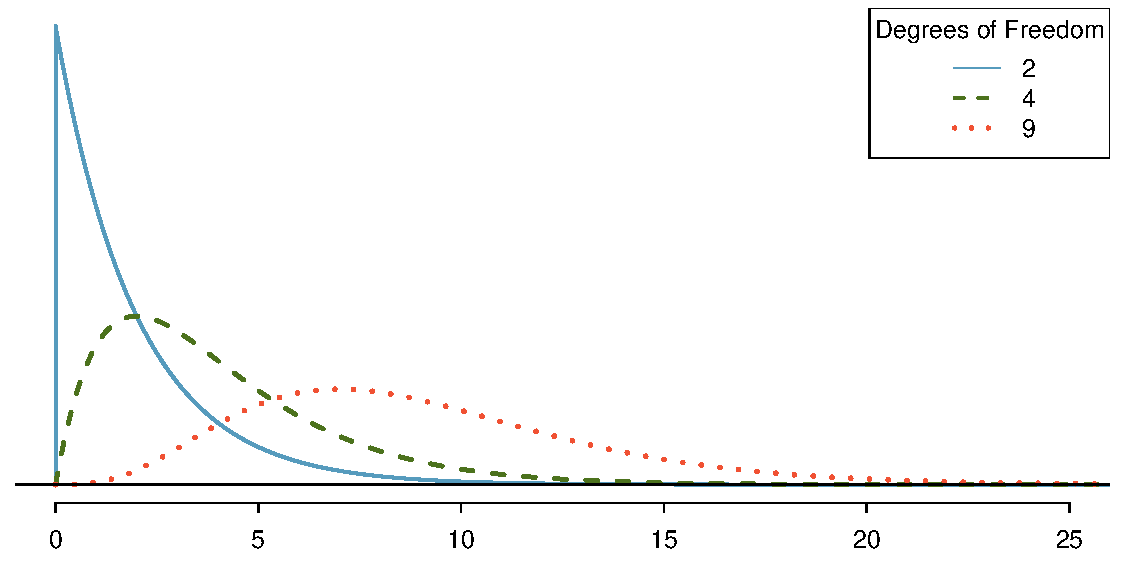
\includegraphics[width=0.8\textwidth]{figures/chiSquareDistributionWithInceasingDF/chiSquareDistributionWithInceasingDF}
			\label{chiSquareDistributionWithInceasingDF}
			\end{figure}
			\textbf{Degrees of freedom:} $df=k-1,$ where $k$ is the number of bins.
		\end{frame}
		\begin{frame}{Chi-Square Tests}
			\begin{itemize}
			\item $X^2=5.89$
			\item $df=3-1=2$
			\item $p-value=$
			\item The data do not provide convincing evidence of racial bias in the juror selection.
		\end{itemize}
		\end{frame}
		\begin{frame}{Chi-Square distributions}
			\textbf{Chi-square test}
			\begin{itemize}
				\item $k$ categories
				\item Observed counts $O_1$, $O_2$, ..., $O_k$
				\item Expected counts $E_1$, $E_2$, ..., $E_k$
				\end{itemize} 
				\textbf{Test statistic}
			\begin{align*}
			x^2 = \frac{(O_1 - E_1)^2}{E_1} + \frac{(O_2 - E_2)^2}{E_2} + \cdots + \frac{(O_k - E_k)^2}{E_k},
			\end{align*}
			where $X^2$ follows the Chi-square distribution with $df=k-1.$
			\vspace{0.3cm}
			$p-value=P(X^2>x^2)$
		\end{frame}
		\begin{frame}{Chi-square Test}
			\textbf{Conditions}
			\begin{itemize}
			\item Independence.
			\item Sample size / distribution. Each particular scenario (i.e. cell count) must have at least 5~expected cases.
			\item Degrees of freedom: $df\geq 2$
		\end{itemize}
		\end{frame}
			\begin{frame}{Chi-Square tests}
				\textbf{Google Experiment}\\
				\begin{itemize}
					\item Test three algorithms using a sample of 10,000 google.com search queries.
				\item Breakdown of test subjects into three search groups.
			\end{itemize}
				\begin{table}[h]
				\centering
				\resizebox{0.8\textwidth}{!}{
				\begin{tabular}{ll ccc ll}
				\hline
				Search algorithm	 & \hspace{1mm} & current & test 1 & test 2 & \hspace{1mm} & Total \\
				Counts &		& 5000 & 2500 & 2500 & & 10000 \\
				\hline
				\end{tabular}}
				\end{table}
			\end{frame}
			\begin{frame}{Chi-Square tests}
				\textbf{Q:} Do the results align with the user's interest?\\
				
				\textbf{Quantifying the result}
				 \begin{enumerate}
					\item The user clicked one of the links provided and did not try a new search or \item The user performed a related search.
				\end{enumerate}
			\end{frame}
				\begin{frame}{Chi-Square tests}
					Results of the Google search algorithm experiment.
				\begin{table}[h]
				\centering\resizebox{0.7\textwidth}{!}{
				\begin{tabular}{ll ccc ll}
				\hline
				Search algorithm & \hspace{1mm} & current & test 1 & test 2 & \hspace{1mm} & Total \\
				\hline
				No new search				   & & 3511    & 1749 & 1818 & 				& 7078 \\
				New search				   & & 1489    & 751	& 682    &				& 2922 \\
				\hline
				Total						   & & 5000    & 2500 & 2500 & 				& 10000 \\
				\hline
				\end{tabular}}
				
				\end{table}
			\end{frame}
			\begin{frame}{Chi-Square tests}
				\textbf{Testing for independence}
				\begin{itemize}
				\item[$H_0$:] The algorithms each perform equally well.
				\item[$H_A$:] The algorithms do not perform equally well.
				\end{itemize}
			\end{frame}
			\begin{frame}{Chi-Square tests}
				\begin{itemize}
					\item $r\times c$ categories, $r$ and $c$ are number of rows and columns respectively
					\item Observed counts $O_1$, $O_2$, ..., $O_{r\cdot c}$
					\item Expected counts $E_1$, $E_2$, ..., $E_{r\cdot c}$
					\end{itemize} 
					\textbf{Test statistic}
				\begin{align*}
				x^2 = \frac{(O_1 - E_1)^2}{E_1} + \frac{(O_2 - E_2)^2}{E_2} + \cdots + \frac{(O_{r\cdot c} - E_{r\cdot c})^2}{E_{r\cdot c}},
				\end{align*}
				where $X^2$ follows the Chi-square distribution with $df=(r-1)(c-1).$
				
				\vspace{0.3cm}
				$p-value=P(X^2>x^2)$
			\end{frame}
			\begin{frame}{Chi-Square tests}
				\textbf{Computing expected counts in a two-way table}\\
				To identify the expected count for the $i^{th}$ row and $j^{th}$ column, compute
				$$\text{Expected Count}_{\text{row }i,\text{ col }j} = \frac{(\text{row $i$ total}) \times  (\text{column $j$ total})}{\text{table total}}\vspace{2mm}$$
			\end{frame}
				\begin{frame}{Chi-Square tests}
					The observed counts and the (expected counts).
					\begin{table}[h]
					\centering
					\resizebox{0.9\textwidth}{!}{
					\begin{tabular}{l lll lll lll l}
					\hline
					Search algorithm\hspace{2mm} & \multicolumn{2}{l}{current} &&
										\multicolumn{2}{l}{test 1} &&
										\multicolumn{2}{l}{test 2} & \hspace{0mm} & Total \\
					\hline
					No new search		   & 3511 &\footnotesize(3539)    &&
										1749 &(1769.5)	&&
										1818 &\footnotesize(1769.5) &	& 7078 \\
					New search		   & 1489 &\footnotesize(1461)   && 
										751 &\footnotesize(730.5)	&& 
										682 &\footnotesize(730.5)    &		& 2922 \\
					\hline
					Total				   & 5000 &&& 	2500 &&& 	2500 &&& 	10000 \\
					\hline
					\end{tabular}}
					\end{table}
					\begin{itemize}
					\item $X^2 = 6.120$
					\item $df = (2-1)\times (3-1) = 2$
					\item $p-value<0.05$
					\item The data provide convincing evidence that there is some difference in performance among the algorithms.
				\end{itemize}
				\end{frame}
\end{document}